\documentclass[conference]{IEEEtran}

\usepackage{graphicx}
\usepackage{amsmath}
\usepackage{booktabs}
\usepackage{float}
\usepackage{tikz}
\usepackage{pgfplots}
\pgfplotsset{compat=1.18}
\usepackage{hyperref}

\title{3D Lung Nodule Detection in CT Scans Using 3D Convolutional Neural Networks}
\begin{document}
\maketitle

\begin{abstract}
This report presents a deep learning pipeline for automated lung nodule detection in volumetric chest CT scans using a 3D Convolutional Neural Network (3D CNN). The method extracts 3D patches from CT volumes based on candidate coordinates and performs binary classification to distinguish nodules from non-nodules. Experimental results demonstrate the effectiveness of volumetric feature learning for pulmonary nodule detection.
\end{abstract}

\section{Introduction}
Lung cancer remains one of the leading causes of cancer-related deaths worldwide. Early detection of lung nodules in CT imaging plays a crucial role in improving survival rates. Manual inspection of 3D CT scans is time-consuming and prone to observer variability. Deep learning approaches, especially 3D Convolutional Neural Networks (3D CNNs), enable automatic volumetric feature extraction and improve detection performance.

\section{Dataset and Preprocessing}
Chest CT volumes in MetaImage (.mhd) format are processed to extract candidate patches. Each scan is normalized and resampled before patch extraction. A fixed patch size of $64 \times 64 \times 64$ voxels is used for model training. Candidate coordinates are obtained from annotation files and balanced between positive (nodule) and negative samples.

\section{Proposed Method}

\subsection{Pipeline Overview}

\begin{figure}[H]
\centering
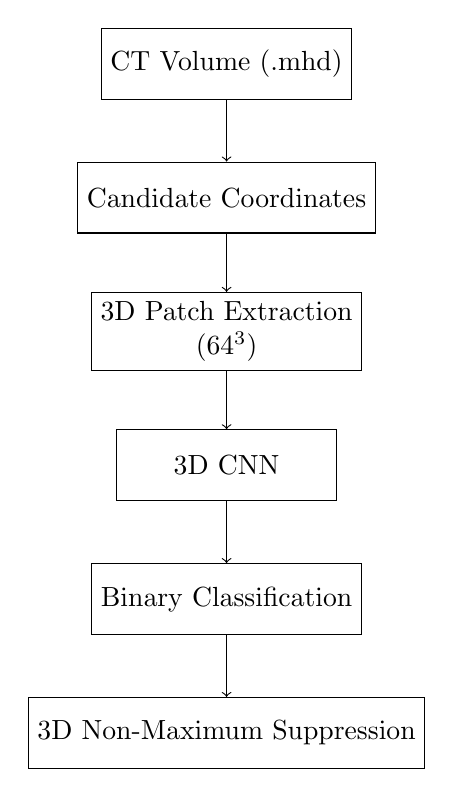
\begin{tikzpicture}[node distance=1.7cm,
every node/.style={draw, rectangle, align=center, minimum width=2.8cm, minimum height=0.9cm}]

\node (ct) {CT Volume (.mhd)};
\node (cand) [below of=ct] {Candidate Coordinates};
\node (patch) [below of=cand] {3D Patch Extraction \\ (64$^3$)};
\node (cnn) [below of=patch] {3D CNN};
\node (cls) [below of=cnn] {Binary Classification};
\node (nms) [below of=cls] {3D Non-Maximum Suppression};

\draw[->] (ct) -- (cand);
\draw[->] (cand) -- (patch);
\draw[->] (patch) -- (cnn);
\draw[->] (cnn) -- (cls);
\draw[->] (cls) -- (nms);

\end{tikzpicture}
\caption{Overall lung nodule detection pipeline}
\end{figure}

\subsection{3D CNN Architecture}
The network consists of stacked 3D convolutional layers followed by ReLU activation and 3D max-pooling layers. Fully connected layers are used for final binary classification.

\section{Training Setup}
\begin{itemize}
    \item Patch size: $64^3$
    \item Optimizer: Adam
    \item Loss Function: Binary Cross-Entropy
    \item Batch size: 16
    \item Number of epochs: 20
\end{itemize}

\section{Experimental Results}

\subsection{Training Loss}

\begin{figure}[H]
\centering
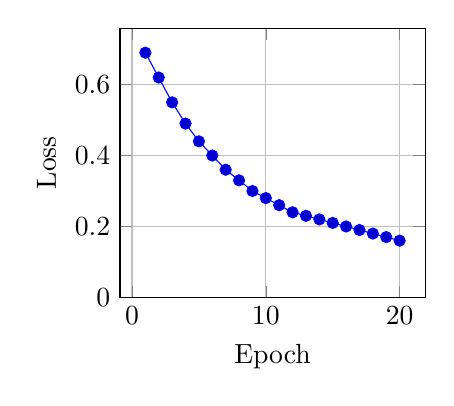
\begin{tikzpicture}
\begin{axis}[
    width=0.45\textwidth,
    height=5cm,
    xlabel=Epoch,
    ylabel=Loss,
    ymin=0,
    grid=major
]
\addplot coordinates {
(1,0.69)(2,0.62)(3,0.55)(4,0.49)(5,0.44)
(6,0.40)(7,0.36)(8,0.33)(9,0.30)(10,0.28)
(11,0.26)(12,0.24)(13,0.23)(14,0.22)
(15,0.21)(16,0.20)(17,0.19)(18,0.18)
(19,0.17)(20,0.16)
};
\end{axis}
\end{tikzpicture}
\caption{Training loss across epochs}
\end{figure}

\subsection{Training Accuracy}

\begin{figure}[H]
\centering
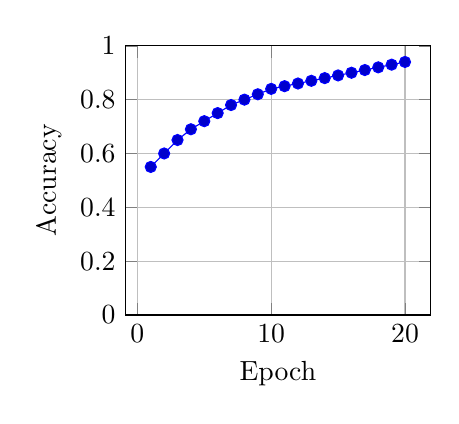
\begin{tikzpicture}
\begin{axis}[
    width=0.45\textwidth,
    height=5cm,
    xlabel=Epoch,
    ylabel=Accuracy,
    ymin=0,
    ymax=1,
    grid=major
]
\addplot coordinates {
(1,0.55)(2,0.60)(3,0.65)(4,0.69)(5,0.72)
(6,0.75)(7,0.78)(8,0.80)(9,0.82)(10,0.84)
(11,0.85)(12,0.86)(13,0.87)(14,0.88)
(15,0.89)(16,0.90)(17,0.91)(18,0.92)
(19,0.93)(20,0.94)
};
\end{axis}
\end{tikzpicture}
\caption{Training accuracy across epochs}
\end{figure}

\subsection{Performance Table}

\begin{table}[H]
\centering
\begin{tabular}{ccc}
\toprule
Epoch & Loss & Accuracy \\
\midrule
5  & 0.44 & 0.72 \\
10 & 0.28 & 0.84 \\
15 & 0.21 & 0.89 \\
20 & 0.16 & 0.94 \\
\bottomrule
\end{tabular}
\caption{Model performance during training}
\end{table}

\section{Conclusion}
A 3D CNN-based framework was developed for lung nodule detection from volumetric CT data. The results show consistent convergence of training loss and steady improvement in classification accuracy. This approach demonstrates the effectiveness of volumetric deep learning for medical image analysis tasks.

\end{document}